\documentclass[conference]{IEEEtran}
\IEEEoverridecommandlockouts
% The preceding line is only needed to identify funding in the first footnote. If that is unneeded, please comment it out.
%Template version as of 6/27/2024

\usepackage{cite}
\usepackage{amsmath,amssymb,amsfonts}
\usepackage{algorithmic}
\usepackage{graphicx}
\usepackage{textcomp}
\usepackage{xcolor}
\usepackage{glossaries}
\usepackage{url}
\usepackage{adjustbox}      % for scaling tables
\usepackage[table]{xcolor} % To color rows in a table

\usepackage{tabularx}
\usepackage[margin=1in]{geometry}
% \usepackage[
%     colorlinks=true,      % Use colored text instead of boxes
%     linkcolor=black,       % Color for internal links (e.g., table of contents)
%     citecolor=black,       % Color for citations
%     urlcolor=blue,        % Color for URLs
%     filecolor=blue,       % Color for file links
%     menucolor=blue,       % (optional) Color for Acrobat menu items
%     linktoc=all,          % Color both the section and page number in TOC
%     pdfborder={0 0 0}     % No border around links
% ]{hyperref}


% Glossaries Configuration
\newacronym{3gpp}{3GPP}{3rd Generation Partnership Project}
\newacronym{5g}{5G}{Fifth-Generation}
\newacronym{5gc}{5GC}{5G Core}
\newacronym{6g-ia}{6G-IA}{6G Smart Networks and Services Industry Association}
\newacronym{6g}{6G}{Sixth-Generation}
\newacronym{a2a}{A2A}{Automatic to Autonomous}
\newacronym{ai}{AI}{Artificial Intelligence}
\newacronym{ai/ml}{AI/ML}{Artificial Intelligence and Machine Learning}
\newacronym{aiops}{AIOps}{Artificial Intelligence for IT Operations}
\newacronym{anm}{ANM}{Autonomic Network Management}
\newacronym{api}{API}{Application Programmable Interface}
\newacronym{asic}{Application-specific Integrated Circuits}{ASIC}
\newacronym{b5g}{B5G}{Beyond 5G}
\newacronym{bsa}{BSA}{Back-Situation Awareness}
\newacronym{cam}{CAM}{Cooperative Awareness Message}
\newacronym{capex}{CAPEX}{Capital expenditure }
\newacronym{cdn}{CDN}{Content Delivery Network}
\newacronym{cdnaas}{CDNaaS}{CDN as a Service}
\newacronym{cits}{C-ITS}{Cooperative Intelligent Transport System}
\newacronym{cmeao}{cMEAO}{Centralized MEC Application Orchestrator}
\newacronym{cmi}{CMI}{Campus Middelheim}
\newacronym{cn}{CN}{Core Network}
\newacronym{cnl}{CNL}{Constrained Natural Language}
\newacronym{cp}{CP}{Control Plane}
\newacronym{cpu}{CPU}{Central Processing Unit}
\newacronym{csi}{CSI}{Channel State Information}
\newacronym{dasa}{DASA}{Dynamic Auto-Scaling Algorithm}
\newacronym{ddos}{DDoS}{Distributed DoS}
\newacronym{denm}{DENM}{Decentralized Environmental Notification Message}
\newacronym{dl}{DL}{Deep Learning}
\newacronym{dos}{DoS}{Denial of Service}
\newacronym{dqn}{DQN}{Deep Q-Network}
\newacronym{drl}{DRL}{Deep Reinforcement Learning}
\newacronym{e2e}{E2E}{End-to-End}
\newacronym{edgeapps}{EdgeApps}{Edge Network Applications}
\newacronym{embb}{eMBB}{enhanced Mobile Broadband}
\newacronym{eni}{ENI}{Experiential Networked Intelligence}
\newacronym{etsi}{ETSI}{European Telecommunications Standards Institute}
\newacronym{eu}{EU}{European Union}
\newacronym{fl}{FL}{Federated Learning}
\newacronym{gcm}{gCM}{Next-Generation Crowdsourcing Metric}
\newacronym{ghg}{GHG}{Global Greenhouse Gas}
\newacronym{gpcu}{GPCU}{General Purpose Computing Unit}
\newacronym{gps}{GPS}{Global Positioning System}
\newacronym{gpu}{GPU}{Graphic Processing Unit}
\newacronym{gui}{GUI}{Graphical User Interface}
\newacronym{hap}{HAP}{High-Altitude Platform}
\newacronym{ibn}{IBN}{Intent-Based Networking}
\newacronym{ict}{ICT}{Information and Communication Technology}
\newacronym{idm}{IDM}{Intent-Driven Management}
\newacronym{iga}{IGA}{Iterative Gradient Attack}
\newacronym{iiot}{IIoT}{Industrial Internet of Things}
\newacronym{ime}{IME}{Intent Management Entity}
\newacronym{imf}{IMF}{Intent Management Function}
\newacronym{iot}{IoT}{Internet-of-Things}
\newacronym{ip}{IP}{Internet Protocol}
\newacronym{ipmi}{IPMI}{Intelligent Platform Management Interface}
\newacronym{isg}{ISG}{Industry Specification Group}
\newacronym{its-g5}{ITS-G5}{Intelligent Transportation System}
\newacronym{itu}{ITU}{International Telecommunications Union}
\newacronym{ju}{JU}{Joint Undertaking}
\newacronym{k8s}{K8s}{Kubernetes}
\newacronym{kpi}{KPI}{Key Performance Indicator}
\newacronym{kv}{KV}{Key Value}
\newacronym{kvi}{KVI}{Key Value Indicator}
\newacronym{lap}{LAP}{Low-Altitude Platform}
\newacronym{lc}{LC}{Life-cycle}
\newacronym{lcm}{LCM}{Life Cycle Management}
\newacronym{leo}{LEO}{Low-Earth Orbit}
\newacronym{lidar}{LiDAR}{Light Detection and Ranging}
\newacronym{llm}{LLM}{Large Language Model}
\newacronym{m2m}{M2M}{Machine-To-Machine}
\newacronym{mano}{MANO}{MANagement and Orchestration}
\newacronym{mape-k}{MAPE-K}{Monitor-Analyze-Plan-Execute-Knowledge}
\newacronym{mcdm}{MCDM}{Multi-Criteria Decision-Making}
\newacronym{mcs}{MCS}{Mission-critical service}
\newacronym{md}{MD}{Management Domain}
\newacronym{mec}{MEC}{Multi-Access Edge Computing}
\newacronym{mitm}{MITM}{Man-In-The-Middle}
\newacronym{ml}{ML}{Machine Learning}
\newacronym{mmg}{MMG}{Monitoring Model Generator}
\newacronym{mmtc}{mMTC}{massive Machine-Type Communication}
\newacronym{mno}{MNO}{Mobile Network Operator}
\newacronym{mse}{MSE}{Mean Squared Error}
\newacronym{nbi}{NBI}{Northbound Interface}
\newacronym{nfv}{NFV}{Network Function Virtualization}
\newacronym{nfvi-i}{NFVI-I}{Infrastructure in Italy}
\newacronym{nfvi-o}{NFVI-O}{Infrastructure in Romania}
\newacronym{nfvi}{NFVI}{Network Function Virtualization Infrastructure}
\newacronym{ni}{NI}{Network Infrastructure}
\newacronym{nif}{NIF}{Network Intelligent Function}
\newacronym{noc}{NoC}{Network On-chip}
\newacronym{npu}{NPU}{Neural Processing Unit}
\newacronym{ns}{NS}{Network Slicing}
\newacronym{nsa}{NSA}{None-Standalone Architecture}
\newacronym{o-ran}{O-RAN}{Open RAN}
\newacronym{obu}{OBU}{On-board Unit}
\newacronym{ooda}{OODA}{Observe-Orient-Decide-Act}
\newacronym{opex}{OPEX}{Operational expenditure}
\newacronym{pdu}{PDU}{Power Distribution Unit}
\newacronym{poc}{PoC}{Proof-of-Concept}
\newacronym{pop}{PoP}{Point of Presence}
\newacronym{prb}{PRB}{Physical Resource Block}
\newacronym{qod}{QoD}{Quality on Demand}
\newacronym{qoe}{QoE}{Quality of Experience}
\newacronym{qos}{QoS}{Quality of Service}
\newacronym{ran}{RAN}{Radio Access Network}
\newacronym{rapl}{RAPL}{Running Average Power Limit}
\newacronym{rbf}{RBF}{Radial Basis Function}
\newacronym{rd}{R\&D}{Research and Development}
\newacronym{rest}{REST}{REpresentational State Transfer}
\newacronym{ric}{RIC}{RAN Intelligent Controller}
\newacronym{rl}{RL}{Reinforcement Learning}
\newacronym{rsrp}{RSRP}{Reference Signal Received Power}
\newacronym{rsrq}{RSRQ}{Reference Signal Received Quality}
\newacronym{rsu}{RSU}{Roadside Unit}
\newacronym{sa}{SA}{Standalone}
\newacronym{sba}{SBA}{Service-Based Architecture}
\newacronym{sbi}{SBI}{Southbound Interface}
\newacronym{sdg}{SDG}{Sustainable Development Goal}
\newacronym{sdk}{SDK}{Software Development Kit}
\newacronym{sdn}{SDN}{Software Defined Networking}
\newacronym{sdo}{SDO}{Standards Development Organisation}
\newacronym{seal}{SEAL}{Service Enabler Architecture Layer for Verticals}
\newacronym{shw}{SHW}{Smart Highway}
\newacronym{sl}{SL}{Supervised Learning}
\newacronym{sla}{SLA}{Service-Level Agreement}
\newacronym{snmp}{SNMP}{Simple Network Management Protocol}
\newacronym{sns}{SNS}{Smart Network and Services}
\newacronym{sota}{SotA}{State of the Art}
\newacronym{ssla}{SSLA}{Security Service-Level Agreement}
\newacronym{stm}{STM}{Smart Traffic Management}
\newacronym{svr}{SVR}{Support Vector Regression}
\newacronym{tim}{TIM}{Telecom Italia}
\newacronym{tl}{TL}{Transfer Learning}
\newacronym{topsis}{TOPSIS}{The Technique for Order of Preference}
\newacronym{tpu}{TPU}{Tensor Processing Unit}
\newacronym{ue}{UE}{User Equipment}
\newacronym{ul}{UL}{Unsupervised Learning}
\newacronym{un}{UN}{United Nations}
\newacronym{up}{UP}{User Plane}
\newacronym{upf}{UPF}{User Plane Function}
\newacronym{urllc}{URLLC}{Ultra-Reliable Low-Latency Communication}
\newacronym{usrp}{USRP}{Universal Software Radio Peripheral}
\newacronym{ux}{UX}{User eXperience}
\newacronym{v2x}{V2X}{Vehicle-to-Everything}
\newacronym{vae}{VAE}{Vertical Application Enabler}
\newacronym{val}{VAL}{Vertical Application Layer}
\newacronym{vcdn}{vCDN}{virtual Content Delivery Network}
\newacronym{vec}{VEC}{Vehicular Edge Computing}
\newacronym{vm}{VM}{Virtual Machine}
\newacronym{vnf}{VNF}{Virtualized Network Function}
\newacronym{vpn}{VPN}{Virtual Private Network}
\newacronym{vru}{VRU}{Vulnerable Road User}
\newacronym{xaas}{XaaS}{Anything as a service}
\newacronym{xr}{XR}{eXtended Reality}
\newacronym{zsm}{ZSM}{Zero-touch Network and Service Management}
\newacronym{ztc}{ZTC}{Zero-touch Commissioning}
\newacronym{ztm}{ZTM}{Zero-touch Management}
\newacronym{zts}{ZTS}{Zero-touch Service} 

% Reference Configuration
\renewcommand{\citedash}{--}
\renewcommand{\citepunct}{,}
\def\BibTeX{{\rm B\kern-.05em{\sc i\kern-.025em b}\kern-.08em
    T\kern-.1667em\lower.7ex\hbox{E}\kern-.125emX}}
\begin{document}

% Space Configuration
\frenchspacing
\renewcommand{\baselinestretch}{0.87}

\title{Scriptorium}

% \author{Raúl Cuervo Bello\IEEEauthorrefmark{1}, Miguel Camelo\IEEEauthorrefmark{2}, Johann Marquez-Barja\IEEEauthorrefmark{1}, and Nina Slamnik-Kriještorac\IEEEauthorrefmark{1}\\
%     \IEEEauthorrefmark{1} University of Antwerp - imec, IDLab - Faculty of Applied Engineering, Belgium \\ \quad\IEEEauthorrefmark{2} University of Antwerp - imec, IDLab - Department of Computer Science, Belgium}

\maketitle

% \begin{abstract}
Network resiliency is essential for ensuring continuous and reliable service delivery in the face of failures, attacks, or unexpected events. As networks become more complex and critical to daily operations, designing resilient architectures and mechanisms is paramount. This topic explores strategies and technologies that enhance network robustness, including redundancy, fault tolerance, rapid recovery, and adaptive reconfiguration. Emphasis is placed on proactive monitoring, automated response, and the integration of intelligent systems to detect and mitigate disruptions. By advancing network resiliency, organizations can minimize downtime, maintain service quality, and support the evolving demands of modern digital infrastructures.
\end{abstract}
\glsresetall


% \begin{IEEEkeywords}
%     Zero-Touch Management, Energy Efficiency, 6G, Vehicular Networks, Smart Highway, Sustainability, Edge Computing
% \end{IEEEkeywords}
\glsresetall

\begin{abstract}
The exponential growth of connectivity and computing demand has made \gls{nfvi} major contributors to global energy consumption. Conventional network and service deployments, whether based on legacy hardware appliances or \gls{nfvi} stacks, struggle to dynamically provision resources for peak data traffic demand. This results in nearly constant energy consumption even during low-traffic periods, leading to inefficient resource use.
Network softwarization and virtualization have enabled flexible and programmable service deployments, which are beneficial for rapid and dynamic scaling of network functions. This paper validates energy-aware service and network orchestration with a \gls{zsm} framework for autonomous optimization of computing, network, and power resources from \gls{nfvi} on a use case focused on connected mobility, and in particular, smart traffic management. By modeling road traffic based on vehicle count and type and \gls{3gpp} profiles for data formats in vehicular communication scenarios, the \gls{zsm} framework adjusts services and resources to services requirements and to actual demand. Experimental validation on the real-life Smart Highway testbed in Antwerp (Belgium) demonstrates a strong correlation between vehicular traffic and power consumption, supporting the hypothesis that adaptive compute and network resource management reduces unnecessary energy use and advances the vision of sustainable and self optimizing \gls{6g} networks.
\end{abstract}
\glsresetall
\section{Energy-Awareness Experiment 1}\label{awar:1}
This is my starting point \cite{3gpp-ts-22-186,3gpp_ts_26_511_v18_1_0}

Every physical capability of the \gls{rsu} is different from each other in terms of maximum wattage.
When the \glspl{rsu} were stressed based on the amount of vehicles, they have a limit of watts also linked to the CPU consumption.

\begin{table}[htbp]
    \centering
    \caption{Average vehicular counts and power consumption per RSU.}
    \label{tab:rsu-traffic-power}
    \begin{tabular}{|c|cc|cc|}
        \hline
        \textbf{RSU} & \multicolumn{2}{c|}{\textbf{Night (17:00--06:00)}} & \multicolumn{2}{c|}{\textbf{Day (06:00--17:00)}}                        \\
        \cline{2-5}
                     & Vehicles                                           & Power (W)                                        & Vehicles & Power (W) \\
        \hline
        1            & 0                                                  & 59                                               & 4        & 58        \\
        2            & 1                                                  & 55                                               & 7        & 55        \\
        3            & 5                                                  & 56                                               & 23       & 56        \\
        5            & 2                                                  & 51                                               & 7        & 51        \\
        6            & 1                                                  & 60                                               & 5        & 60        \\
        7            & 6                                                  & 61                                               & 16       & 61        \\
        \hline
    \end{tabular}
\end{table}
\begin{table}[!t]
    \centering
    \caption{Location mapping between inductive sensors and \glspl{rsu} to monitor vehicular traffic per \gls{rsu} in the E13 Highway, Antwerp Belgium.}
    \label{tab:location-mapping-rsu}
    \begin{adjustbox}{max width=\columnwidth}
        \begin{tabular}{|l|c|l|l|}
            \hline
            \textbf{\gls{rsu}} & \textbf{Vehicles} & \textbf{RSU Location} & \textbf{Nearest Inductive Sensor} \\
            \hline
            1 & 12 & 51.210575, 4.46655        & 51.21056678, 4.466446158 \\
            3 & 25 & 51.215186667, 4.450568333 & 51.21587307, 4.452993707 \\
            7 & 12 & 51.210616667, 4.480896667 & 51.21066931, 4.480559376 \\
            8 & 26 & 51.211091667, 4.491425    & 51.21127494, 4.491424033 \\
            4 & 16 & 51.21574, 4.457151667     & 51.21577734, 4.457154961 \\
            6 & 16 & 51.211236667, 4.472586667 & 51.21121407, 4.472483657 \\
            \hline
        \end{tabular}
    \end{adjustbox}
\end{table}

Table~\ref{tab:rsu-max-capacity} summarizes the maximum number of users (U) and the corresponding maximum wattage (W) capacity for each \gls{rsu}. As shown, \gls{rsu} 5 supports the highest number of vehicles and reaches a higher power consumption compared to the others. This variation highlights the heterogeneous nature of the \glspl{rsu} in the testbed. Figure~\ref{fig:exp1-figure} visually presents the relationship between the number of vehicles and the power consumption for each \gls{rsu}, illustrating how the power usage increases with the load and reaches a plateau at the maximum capacity.

Max vehicles registered: 39 \gls{rsu} 5
\begin{table}[ht]
    \centering
    \caption{Maximum U and W capacity for each \gls{rsu}.}
    \begin{tabular}{ccc}
        \hline
        \gls{rsu} & Max U & Max W Capacity \\
        \hline
        1         & 27    & 69             \\
        2         & 27    & 67             \\
        3         & 27    & 70             \\
        5         & 36    & 68             \\
        6         & 27    & 77             \\
        7         & 31    & 75             \\
        \hline
    \end{tabular}
    \label{tab:rsu-max-capacity}
\end{table}

\begin{figure}[!htb]
    \centering
    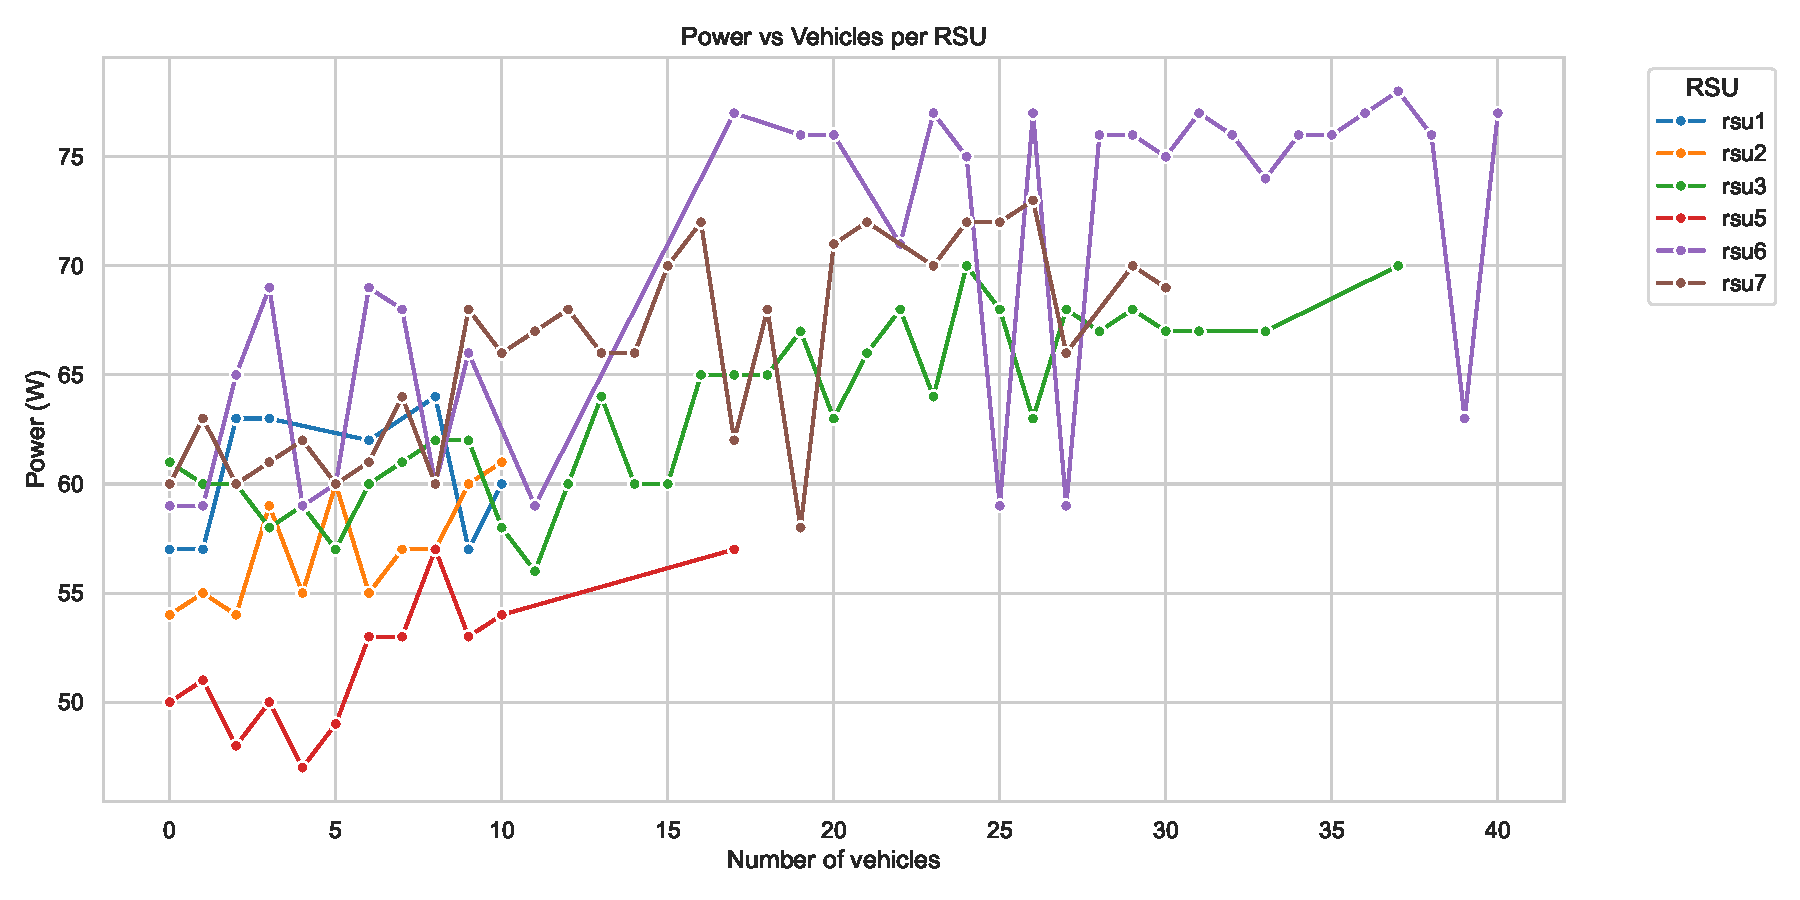
\includegraphics[width=1\columnwidth]{Topics/Energy-Awareness/Figures/power_vehicles_rsu_maximums.pdf}
    \caption{Relationship between the number of vehicles and power consumption for each \gls{rsu}, showing how power usage increases with load and plateaus at maximum capacity.}
    \label{fig:exp1-figure}
\end{figure}
\newpage
\begin{abstract}
Intelligence in Zero-touch Service Management (ZSM) is pivotal for achieving fully autonomous network and service operations. By embedding advanced artificial intelligence (AI) and machine learning (ML) techniques within the ZSM framework, networks can proactively monitor, analyze, and optimize their own performance with minimal human intervention. This enables dynamic adaptation to changing network conditions, efficient resource allocation, and rapid fault detection and resolution. In the context of ZSM, intelligence facilitates closed-loop automation, allowing the system to learn from operational data, predict future states, and make informed decisions to enhance service quality and reliability. As networks evolve towards 6G and beyond, the integration of intelligence in ZSM is essential for supporting complex, heterogeneous environments and delivering on the promise of self-optimizing, resilient, and sustainable network infrastructures.
\end{abstract}
\glsresetall

\section{Intelligence Experiment 1}\label{int:1}
This section presents the first experiment conducted to evaluate the role of intelligence in network automation. The experiment focuses on the integration of artificial intelligence (AI) and machine learning (ML) functions within the Zero-touch Service Management (ZSM) framework. The objective is to assess how these technologies contribute to optimizing network operations and enabling autonomous decision-making processes.

\begin{figure}[!htb]
    \centering
    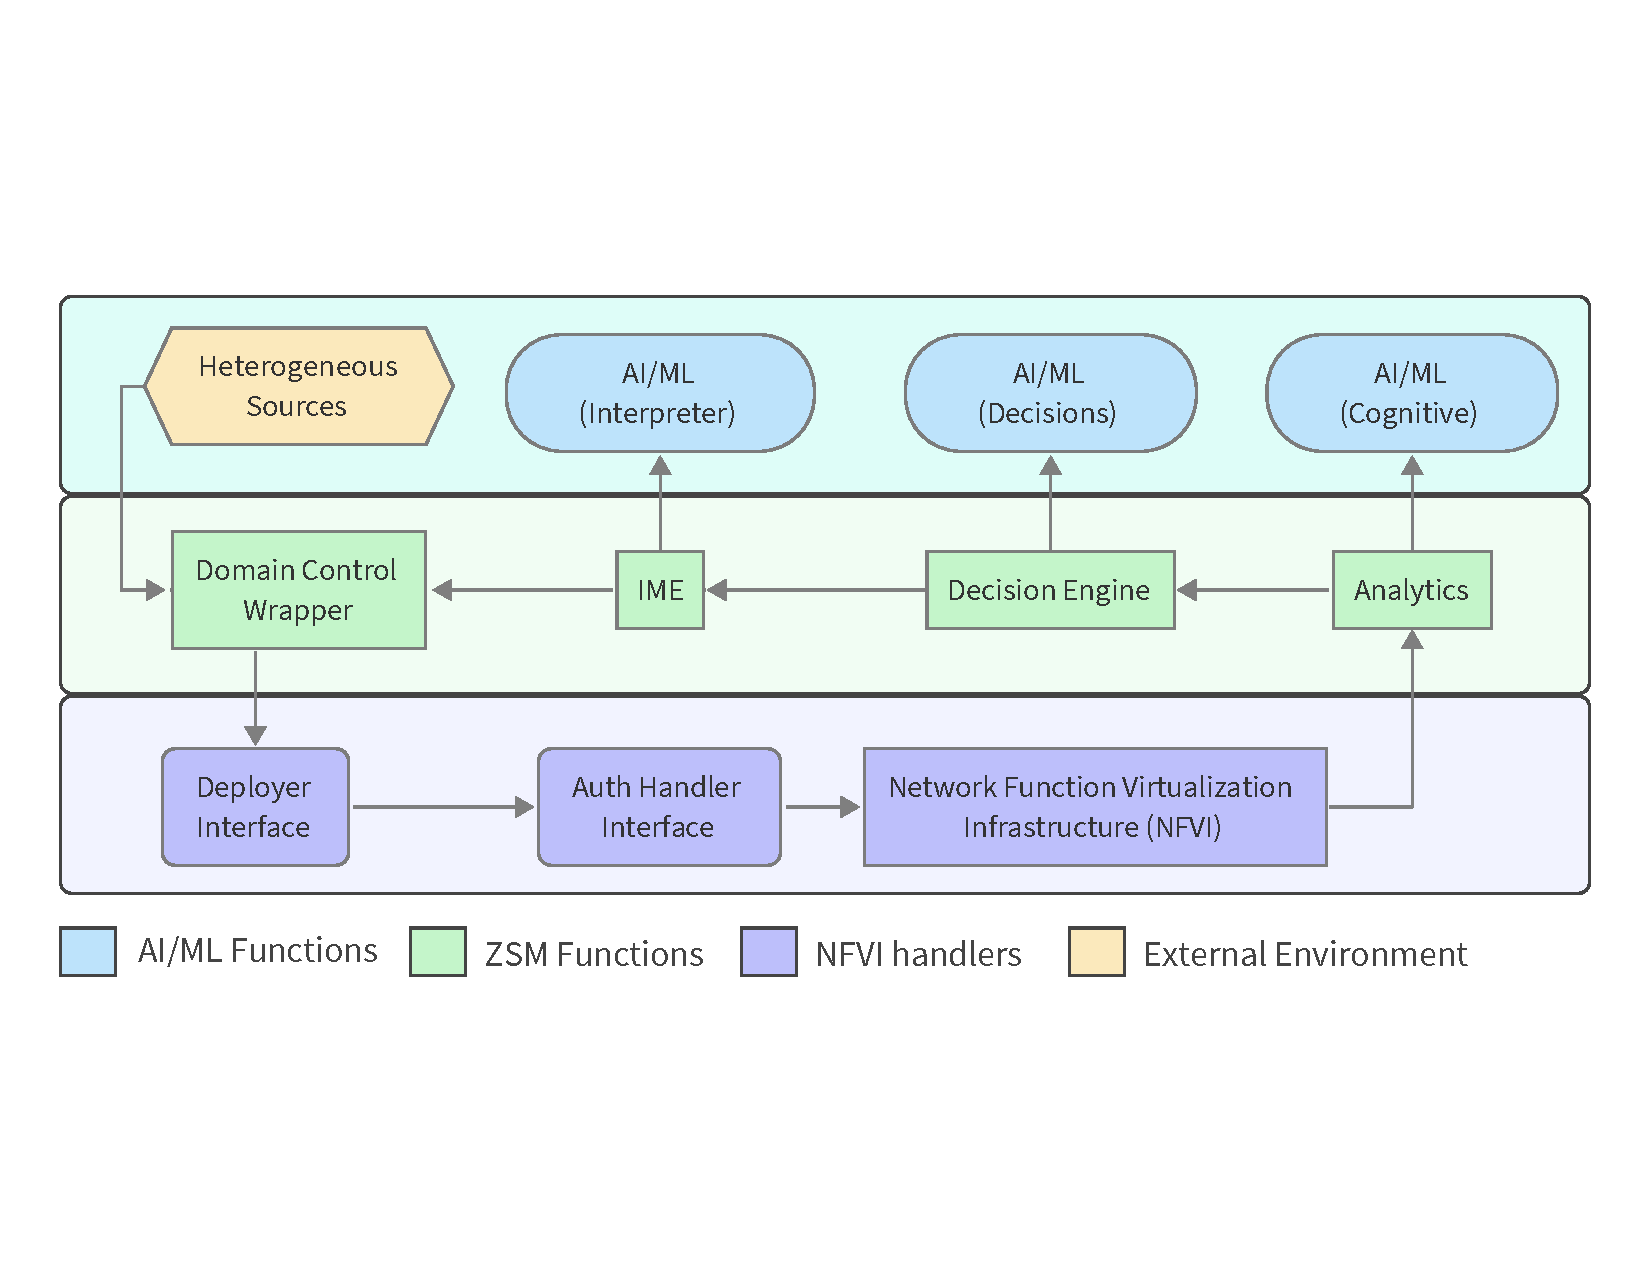
\includegraphics[width=1\columnwidth]{Topics/Intelligence/Figures/AI-ML functions in the ZSM Framework.pdf}
    \caption{AI and ML functions within the ZSM framework, illustrating their role in enhancing network automation and optimization.}
    \label{fig:exp1-figure}
\end{figure}
\newpage
\begin{abstract}
Network resiliency is essential for ensuring continuous and reliable service delivery in the face of failures, attacks, or unexpected events. As networks become more complex and critical to daily operations, designing resilient architectures and mechanisms is paramount. This topic explores strategies and technologies that enhance network robustness, including redundancy, fault tolerance, rapid recovery, and adaptive reconfiguration. Emphasis is placed on proactive monitoring, automated response, and the integration of intelligent systems to detect and mitigate disruptions. By advancing network resiliency, organizations can minimize downtime, maintain service quality, and support the evolving demands of modern digital infrastructures.
\end{abstract}
\glsresetall

\section{Resiliency Experiment 1}\label{res:1}
This section presents the first experiment conducted to evaluate the role of resiliency in network automation. The experiment focuses on the integration of advanced fault tolerance and rapid recovery mechanisms within the Zero-touch Service Management (ZSM) framework. The objective is to assess how these technologies contribute to optimizing network operations and enabling autonomous decision-making processes.
\newpage
\section*{Acknowledgments}\label{sec:Acknowledgments}
This work has been performed within the European projects: SNS JU TrialsNet (Grant Agreement No. 101095871) and 6G-Xcel (Grant Agreement No. 101139194).
This work has been also partially supported by the Flemish Ministry of Mobility and Public Works (MOW) and the regional Agency for Roads and Traffic (AWV), Belgium.

\bibliography{Bibliography/References.bib}
\bibliographystyle{ieeetr}
\definecolor{added}{rgb}{0.9,0.9,1}

\end{document}
